%!TEX root = ../template.tex
%%%%%%%%%%%%%%%%%%%%%%%%%%%%%%%%%%%%%%%%%%%%%%%%%%%%%%%%%%%%%%%%%%%%
%% chapter5.tex
%% NOVA thesis document file
%%
%% Chapter with lots of dummy text
%%%%%%%%%%%%%%%%%%%%%%%%%%%%%%%%%%%%%%%%%%%%%%%%%%%%%%%%%%%%%%%%%%%%

\typeout{NT FILE chapter5.tex}%

\chapter{Tests and Results}
\label{cha:tests_and_results}

\paragraph{}There are two main types of tests that can be performed on the navigation 
system. The first is the path tracking, where the processing time and the time 
to the goal pose are measured. The second is the collision detection to evaluate 
how safe are people or structures near the robot.
Since the navigation system has integrated noise and uncertainty, the test 
results may vary, specially in the real world scenarios where the starting 
and goal poses can be slightly different leading to extremely different results.

\section{Path Tracking Tests}
\label{sec:path_tracking_tests}
There were conducted three tests each with five repetitions to evaluate 
the path tracking performance. The first is a direct path, where the goal is 
posted in front of the robot. The second is a curved path, where the goal is posted 
behind an obstacle but the robot can reach it going forwards. The third and last 
is a recovery test, where the goal is placed to the side of the robot, forcing 
it to go backwards to realign itself. Every test is ran both in a simulation and 
in the corridor environment.

The simulated tests were made in a 13th Gen Intel(R) Core(TM) i9-13900H (2.60 GHz), 32 Gb RAM, 
NVIDIA GeForce RTX 4070 with 12 Gb of VRAM, laptop running Ubuntu 22.04 in wsl2.
Every test is conducted with a 0.8 meters of lookahead distance, a 0.3 m/s maximum linear 
speed and a 0.5 m/s maximum angular speed as the controller parameters, and, 
a turning radius of 1.2 meters, 15 hybrid segments of 10 centimeters each as the 
planner parameters.
Since the simulated environment is totally different form the real world scenarios, 
these tests are not a comparison between the two, but rather a way to evaluate 
the performance of the navigation system in different conditions.
The test goes as follows, first the robot's pose is estimated, this is done by selecting 
the position in the map where the robot is located in RVIZ or by launching the 
navigation stack with the position in the parameters. The latter can only be done 
in simulation due to the certainty of the location where the robot is initialised. It is 
expected that in the real world tests the initial poses estimation will be less 
accurated which will lead to slightly different trajectories even with the same goal 
pose in the map.
\clearpage
\subsection{Direct Path}
\label{subsec:direct_path}
\subsubsection{Simulation Results}

\begin{figure}[h]
    \centering
    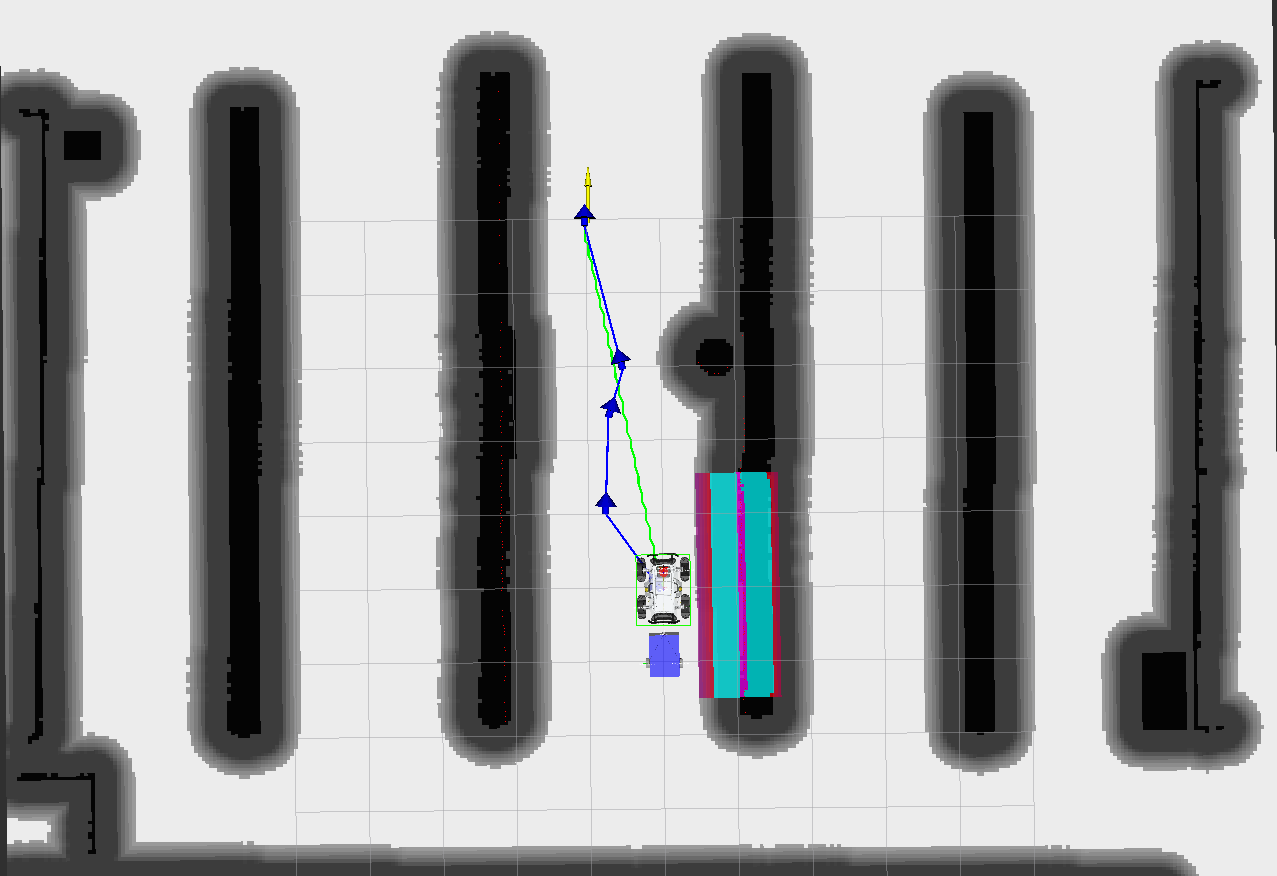
\includegraphics[width=0.95\textwidth]{testdirect.png}
    \caption{Direct path test setup in the simulated environment. Goal pose in yellow.}
    \label{fig:direct_path}
\end{figure}
After five repetitions these were the results obtained in the simulation:

\begin{table}[H]
    \centering
    \begin{tabular}{|c|c|c|}
        \hline
        \textbf{Processing Time (ms)} & \textbf{Dubins Length (m)} & \textbf{Hybrid A* length (m)} \\
        \hline
         16.608 & 5.232 & 0.0  \\
        \hline
         15.653 & 5.232 & 0.0 \\
         \hline
         14.873 & 5.232 & 0.0 \\
         \hline
         16.024 & 5.232 & 0.0 \\
         \hline
         16.411 & 5.232 & 0.0 \\
         \hline
    \end{tabular}
    \caption{Simulation direct path creation results.}
    \label{tab:direct_path_results1}
\end{table}
\begin{table}[H]
    \centering
    \begin{tabular}{|c|c|}
        \hline
        \textbf{Time to goal (s)} & \textbf{Total Length (m)} \\
        \hline
        20.06 & 5.232 \\
        \hline
        19.87 & 5.232 \\
         \hline
         19.54 & 5.232 \\
         \hline
         20.11 & 5.232 \\
         \hline
         19.72 & 5.232 \\
         \hline
    \end{tabular}
    \caption{Simulation direct path tracking results.}
    \label{tab:direct_path_results2}
\end{table}

\clearpage
\subsubsection{Real World Results}
\begin{figure}[h]
    \centering
    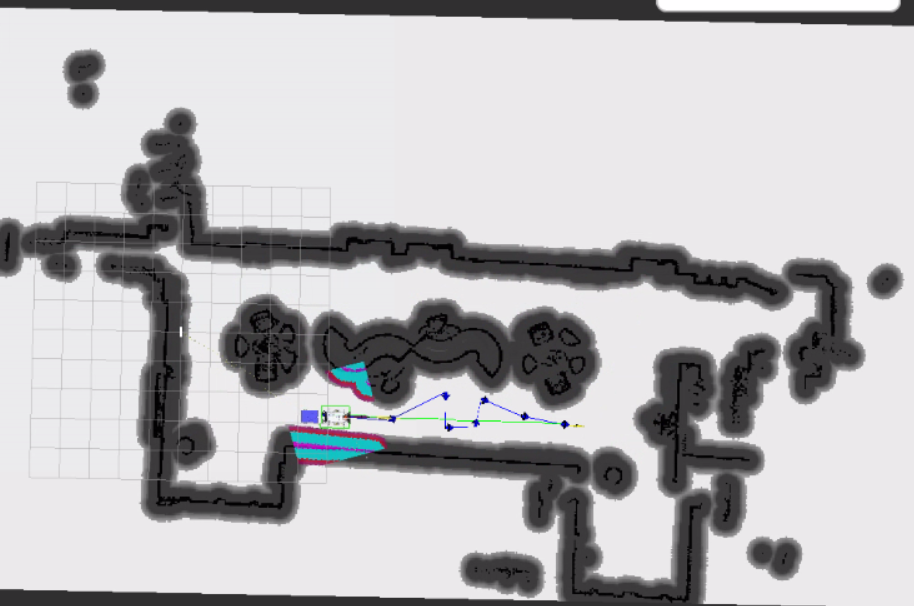
\includegraphics[width=0.95\textwidth]{realonce.png}
    \caption{Direct path test setup in the corridor. Goal pose in yellow.}
    \label{fig:real1}
\end{figure}

After five repetitions these were the results obtained in the corridor:
\begin{table}[H]
    \centering
    \begin{tabular}{|c|c|c|}
        \hline
        \textbf{Processing Time (ms)} & \textbf{Dubins Length (m)} & \textbf{Hybrid A* length (m)} \\
        \hline
         64.011 & 8.88 & 0.0 \\
        \hline
         67.483 & 8.89 & 0.0 \\
         \hline
         55.633 & 8.83 & 0.0 \\
         \hline
         55.864 & 8.88 & 0.0 \\
         \hline
         52.740 & 8.87 & 0.0 \\
         \hline
    \end{tabular}
    \caption{Real world direct path creation results.}
    \label{tab:direct_path_results3}
    
\end{table}
\begin{table}[H]
    \centering
    \begin{tabular}{|c|c|}
        \hline
        \textbf{Time to goal (s)} & \textbf{Total Length (m)} \\
        \hline
        37.92 & 8.88 \\
        \hline
        37.13 & 8.89 \\
         \hline
         38.03 & 8.83 \\
         \hline
         38.19 & 8.88 \\
         \hline
         38.32 & 8.87 \\
         \hline
    \end{tabular}
    \caption{Real world direct path tracking results.}
    \label{tab:direct_path_results4}
\end{table}

The varying lengths of paths are due to real world noise and lack of precision when 
estimating the initial pose of the robot, which lead to slightly different trajectories 
even when the goal pose is the same.
\clearpage

\subsection{Obstructed Path}
\label{subsec:obstructed_path}
\subsubsection{Simulation Results}

\begin{figure}[h]
    \centering
    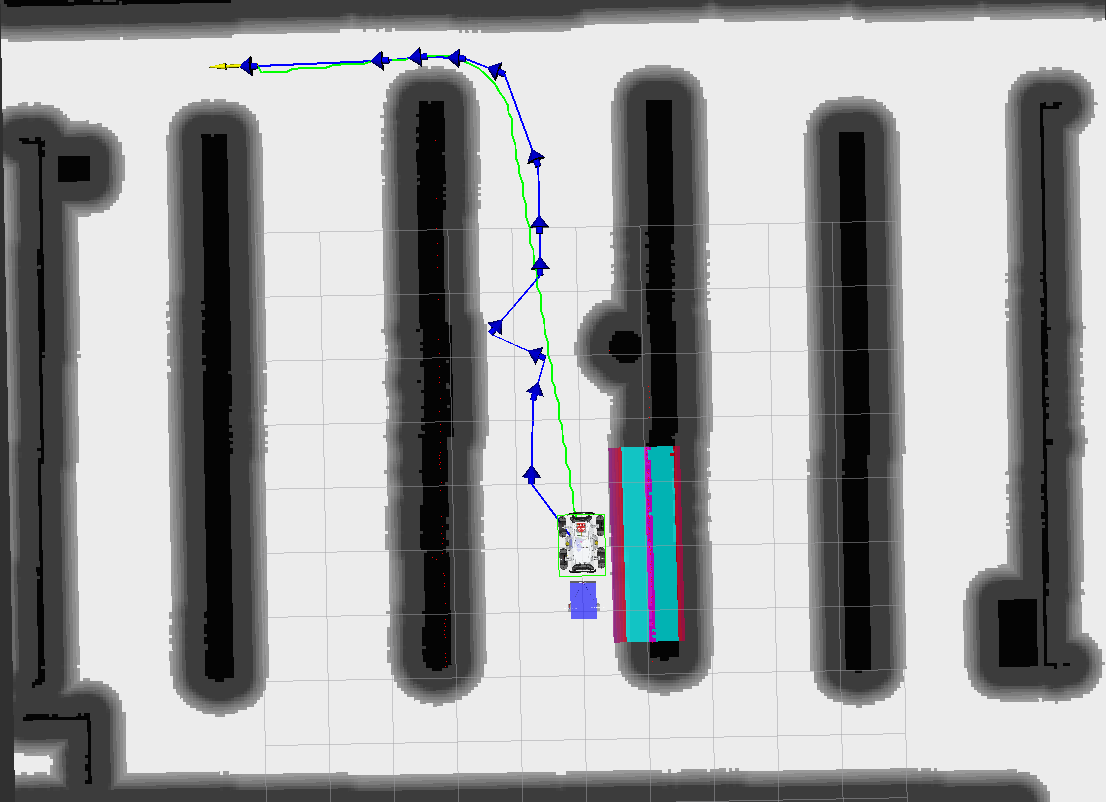
\includegraphics[width=0.95\textwidth]{testobstructed.png}
    \caption{Obstructed path test setup in the simulated environment. Goal pose in yellow.}
    \label{fig:obstructed_path}
\end{figure}

After five repetitions these were the results obtained in the simulation:

\begin{table}[H]
    \centering
    \begin{tabular}{|c|c|c|}
        \hline
        \textbf{Processing Time (ms)} & \textbf{Dubins Length (m)} & \textbf{Hybrid A* length (m)} \\
        \hline
         20.839 & 11.376 & 0.0 \\
        \hline
         17.901 & 11.376 & 0.0 \\
         \hline
         18.050 & 11.376 & 0.0 \\
         \hline
         18.618 & 11.376 & 0.0 \\
         \hline
         18.432 & 11.376 & 0.0 \\
         \hline
    \end{tabular}
    \caption{Simulation obstructed path creation results.}
    \label{tab:obstructed_path_results1}
\end{table}
\begin{table}[H]
    \centering
    \begin{tabular}{|c|c|}
        \hline
        \textbf{Time to goal (s)} & \textbf{Total Length (m)} \\
         \hline
         51.83 & 11.376 \\
         \hline
         50.52 & 11.376 \\
         \hline
         51.45 & 11.376 \\
         \hline
         53.70 & 11.376 \\
         \hline
         52.44 & 11.376 \\
         \hline
    \end{tabular}
    \caption{Simulation obstructed path tracking results.}
    \label{tab:obstructed_path_results2}
\end{table}
\clearpage

\subsubsection{Real World Results}
\begin{figure}[h]
    \centering
    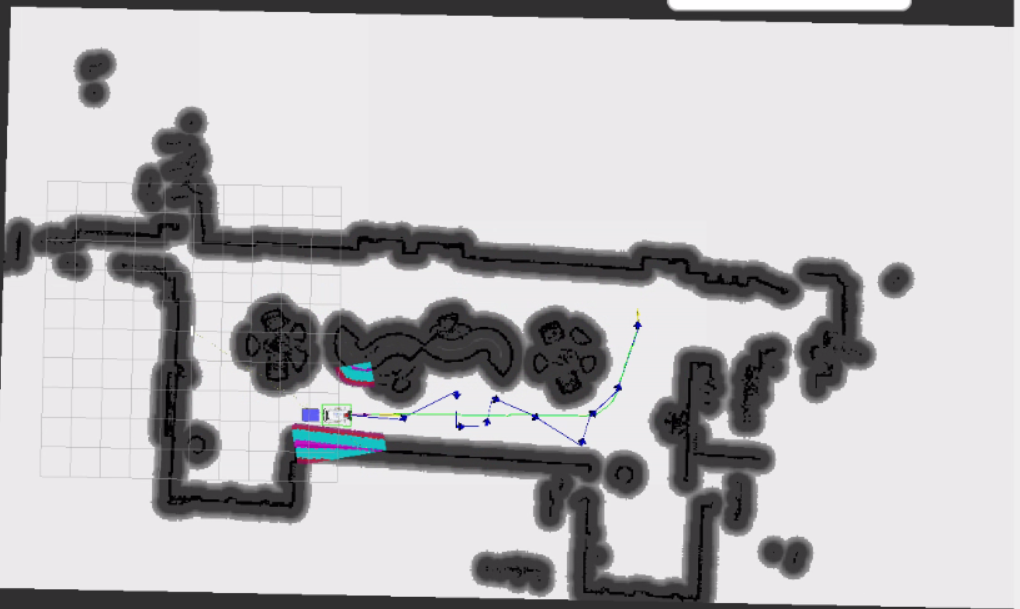
\includegraphics[width=0.95\textwidth]{realtwice.png}
    \caption{Obstructed path test setup in the corridor. Goal pose in yellow.}
    \label{fig:real_obstructed}
\end{figure}

After five repetitions these were the results obtained in the corridor:

\begin{table}[H]
    \centering
    \begin{tabular}{|c|c|c|}
        \hline
        \textbf{Processing Time (ms)} & \textbf{Dubins Length (m)} & \textbf{Hybrid A* length (m)} \\
        \hline
         57.429 & 11.878 & 0.0 \\
        \hline
         56.713 & 11.867 & 0.0 \\
         \hline
         56.720 & 11.880 & 0.0 \\
         \hline
         66.029 & 11.912 & 0.0 \\
         \hline
         66.498 & 11.890 & 0.0 \\
         \hline
    \end{tabular}
    \caption{Real world obstructed path creation results.}
    \label{tab:obstructed_path_results3}
\end{table}
\begin{table}[H]
    \centering
    \begin{tabular}{|c|c|}
        \hline
        \textbf{Time to goal (s)} & \textbf{Total Length (m)} \\
         \hline
         51.83 & 11.878 \\
         \hline
         50.52 & 11.867 \\
         \hline
         51.45 & 11.880 \\
         \hline
         53.70 & 11.912 \\
         \hline
         52.44 & 11.890 \\
         \hline
    \end{tabular}
    \caption{Real world obstructed path tracking results.}
    \label{tab:obstructed_path_results4}
\end{table}

The same reasoning applies to the varying lengths of paths as in the direct 
path test, which is due to real world noise and lack of precision when 
estimating the initial pose of the robot, leading to slightly different trajectories 
even when the goal pose is the same.
\clearpage

\subsection{Recovery test}
\label{subsec:recovery_test}

\subsubsection{Simulation Results}

\begin{figure}[h]
    \centering
    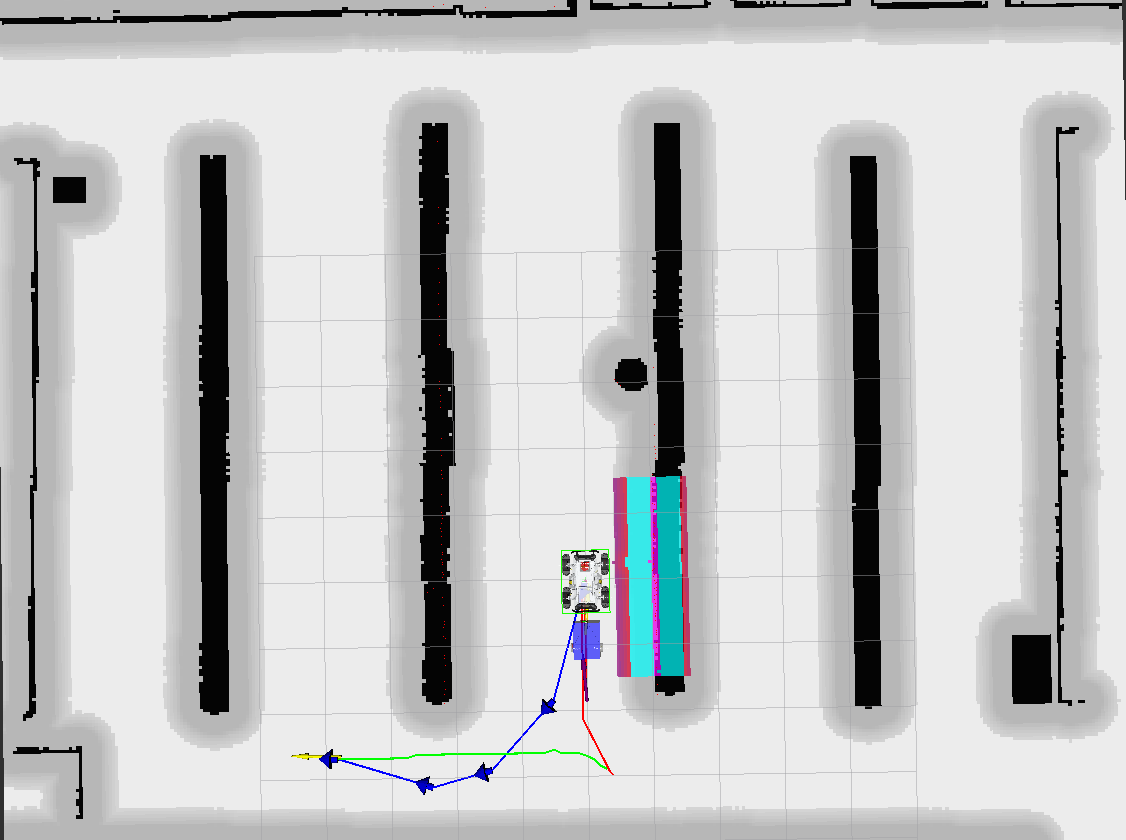
\includegraphics[width=0.95\textwidth]{hybridastarpath1.png}
    \caption{Recovery test setup in the simulated environment. Goal pose in yellow.}
    \label{fig:recovery_test}
\end{figure}
After five repetitions these were the results obtained in the simulation:

\begin{table}[H]
    \centering
    \begin{tabular}{|c|c|c|}
        \hline
        \textbf{Processing Time (ms)} & \textbf{Dubins Length (m)} & \textbf{Hybrid A* length (m)} \\
        \hline
         25.990 & 6.101 & 4.527 \\
        \hline
         25.513 & 6.101 & 4.527 \\
         \hline
         22.841 & 6.101 & 4.527 \\
         \hline
         23.806 & 6.101 & 4.527 \\
         \hline
         22.914 & 6.101 & 4.527 \\
         \hline
    \end{tabular}
    \caption{Simulation recovery creation results.}
    \label{tab:recovery_path_results1}
\end{table}
\begin{table}[H]
    \centering
    \begin{tabular}{|c|c|}
        \hline
        \textbf{Time to goal (s)} & \textbf{Total Length (m)} \\
         \hline
         20.83 & 10.628 \\
         \hline
         20.61 & 10.628 \\
         \hline
         21.14 & 10.628 \\
         \hline
         20.89 & 10.628 \\
         \hline
         20.45 & 10.628 \\
         \hline
    \end{tabular}
    \caption{Simulation recovery tracking results.}
    \label{tab:recovery_path_results2}
\end{table}

\clearpage

\subsubsection{Real World Results}

\paragraph{}In the real world, the recovery test was not very reliable as the recovery 
process varied significantly between trial, however the three trial conducted had the 
following results.
\begin{figure}[h]
    \centering
    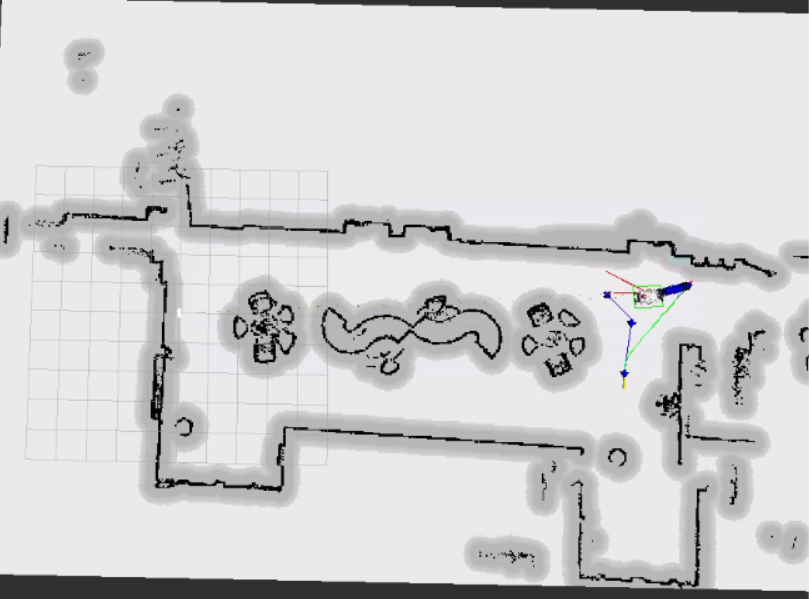
\includegraphics[width=0.85\textwidth]{recovery1.png}
    \caption{Recovery test 1 setup in the real world environment. Goal pose in yellow.}
    \label{fig:real_recovery_test1}
\end{figure}
\begin{figure}[h]
    \centering
    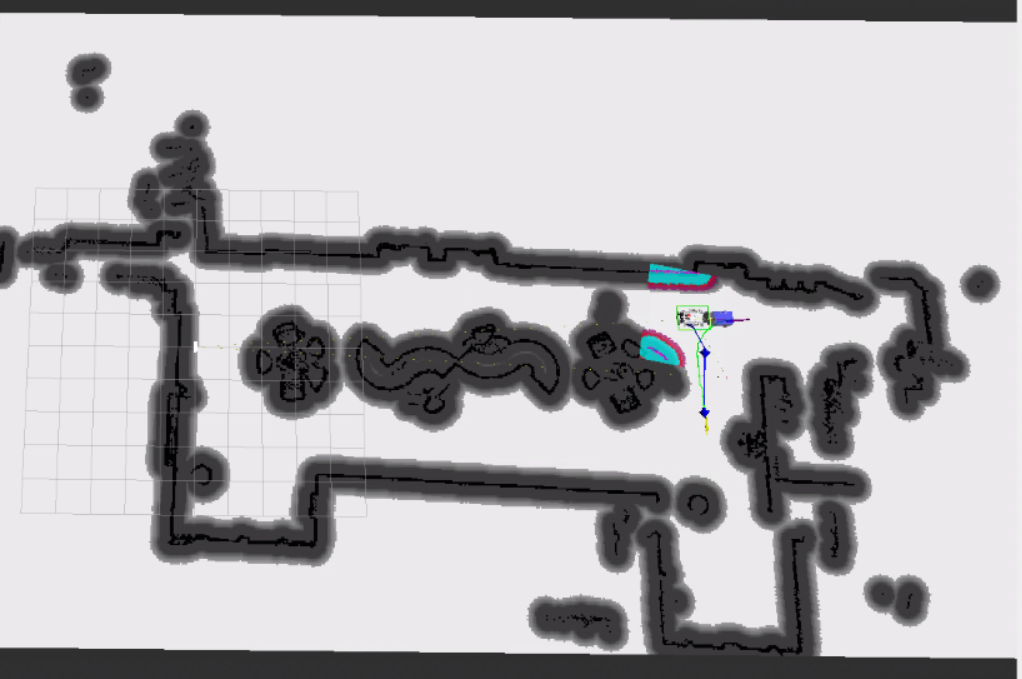
\includegraphics[width=0.85\textwidth]{recovery2.png}
    \caption{Recovery test 2 setup in the real world environment. Goal pose in yellow.}
    \label{fig:real_recovery_test2}
\end{figure}
\clearpage
\begin{figure}[h]
    \centering
    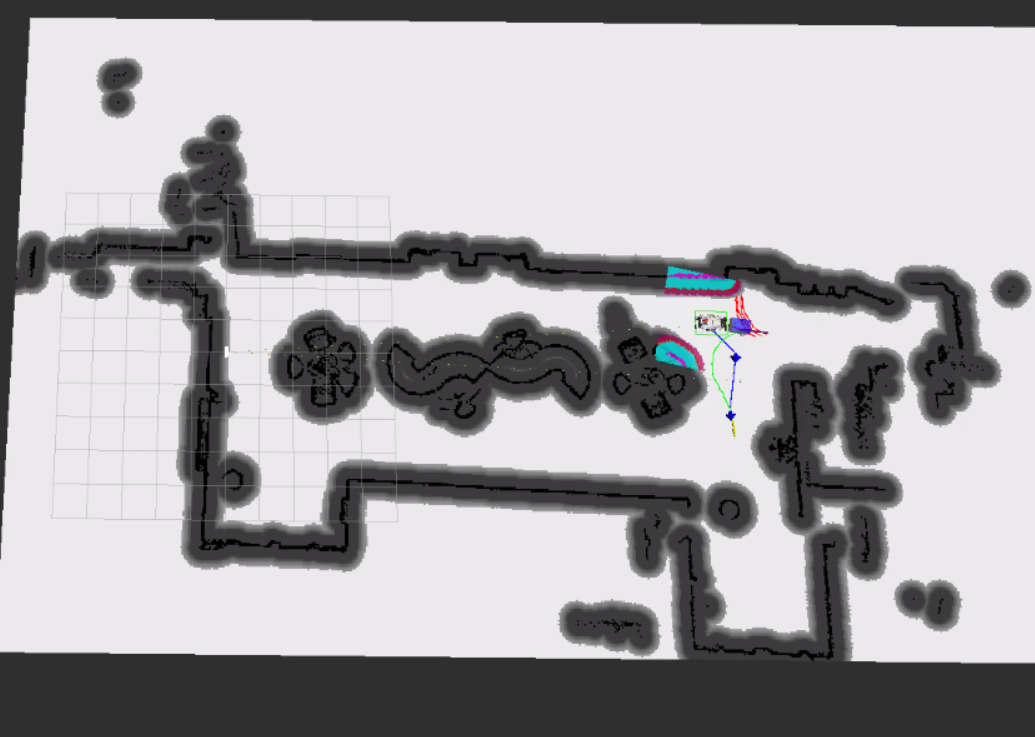
\includegraphics[width=0.85\textwidth]{recovery3.png}
    \caption{Recovery test 3 setup in the real world environment. Goal pose in yellow.}
    \label{fig:real_recovery_test3}
\end{figure}

Note that the difference in color from the first test to the others is simply a 
visualization definition and does not affect any result.

It is possible to verify that the robot, despite being in a similar initial pose 
and trying to achieve a similar goal pose, the planned paths are significantly different, which 
can sometimes lead to the robot not being able to reach due to the path 
having a large amount of recovery turns. However, since the behaviour tree is 
designed to have the planner run every 20 seconds, the planner is sometime able to 
find a more desirable solution while still tracking the first plan. This often 
corrects the initial trajectory, leading to a smoother path. This behaviour was present 
during the third test as it began as a more complex recovery path, but after 
a few seconds the planner found the path in figure \ref{fig:real_recovery_test4}.

Naturally, due to having completely different paths, the processing times and 
lengths of the paths are also different as shown in the tables below.

\begin{table}[H]
    \centering
    \begin{tabular}{|c|c|c|c|}
        \hline
        \textbf{Test} & \textbf{Processing Time (ms)} & \textbf{Dubins Length (m)} & \textbf{Hybrid A* length (m)} \\
        \hline
        1 & 150.990 & 5.126 & 3.418 \\
        \hline
        2 & 121.423 & 3.902 & 2.601 \\
        \hline
        3 & 238.174 & 6.340 & 5.187 \\
        \hline
    \end{tabular}
    \caption{Real world recovery creation results.}
    \label{tab:real_recovery_test_results1}
\end{table}
\begin{table}[H]
    \centering
    \begin{tabular}{|c|c|c|}
        \hline
        \textbf{Test} & \textbf{Time to goal (s)} & \textbf{Total Length (m)} \\
        \hline
        1 & 56.23 & 8.544 \\
        \hline
        2 & 24.35 & 6.503 \\
        \hline
        3 & 32.87 & 11.527 \\
        \hline
    \end{tabular}
    \caption{Real world recovery tracking results.}
    \label{tab:real_recovery_test_results2}
\end{table}


\begin{figure}[h]
    \centering
    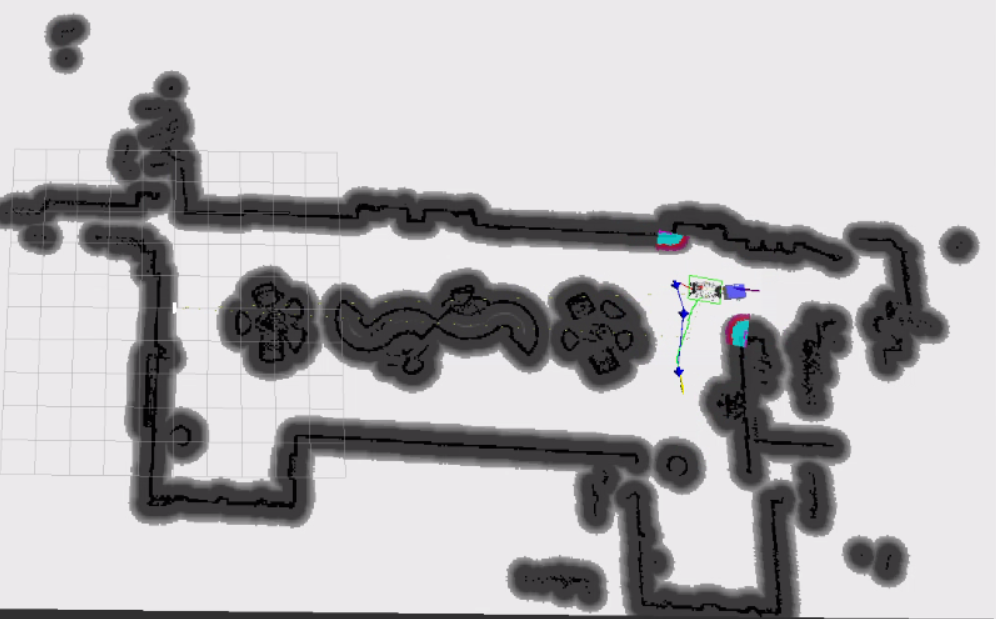
\includegraphics[width=0.85\textwidth]{recoverysquared.png}
    \caption{Recovery correction of the third test setup in the real world environment. Goal pose in yellow.}
    \label{fig:real_recovery_test4}
\end{figure}

\section{Obstacle detection Tests}
\label{sec:obstacle_detection_tests}
\paragraph{}The obstacle detection tests were also conducted in the simulated environment 
and the real world, however, instead of running it in the corridor, it was run 
in the concealed room as it had more obstacles and possibility of dynamic obstacles.

\subsection{Simulation Results}
\paragraph{} The simulation tests were conducted by moving an obstacle in the 
gazebo environment and checking if the robot was able to detect it and stop 
before colliding with it. This was achieved by giving the robot an achievable 
goal pose and moving the obstacle in front while the robot is following the path.

For this test the parameterised range was one meter.

\begin{figure}[h]
    \centering
    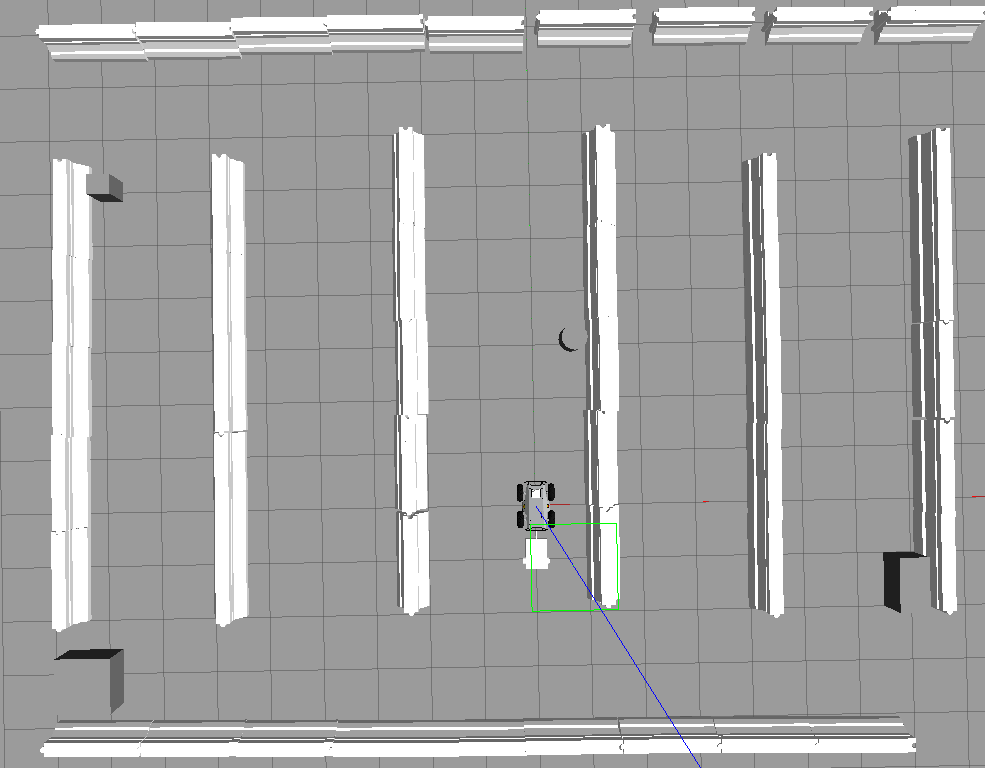
\includegraphics[width=0.85\textwidth]{initial_pose.png}
    \caption{Initial configuration in the simulated environment.}
    \label{fig:sim_obstacle_detection1}
\end{figure}
\begin{figure}[h]
    \centering
    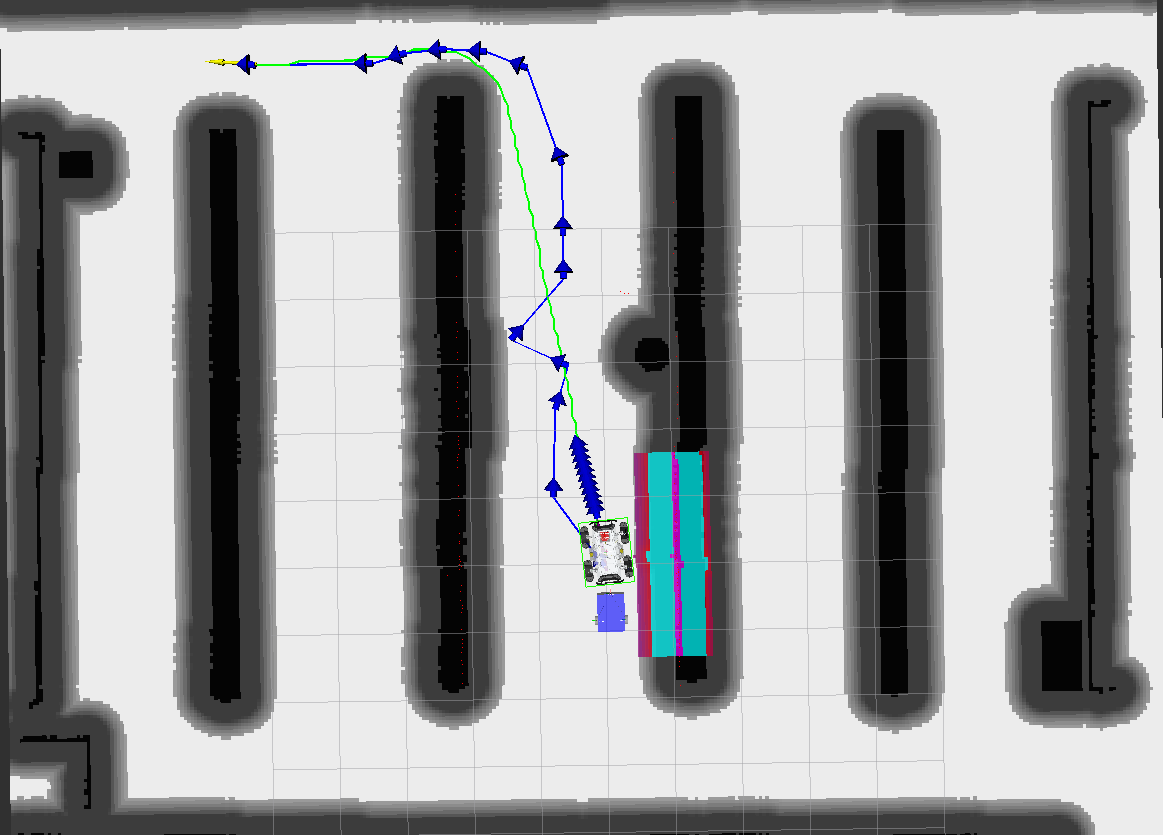
\includegraphics[width=0.85\textwidth]{initial_path.png}
    \caption{Initial path in the simulated environment. The blue arrows coming out from the tractor represent the collision detection range.}
    \label{fig:sim_obstacle_detection2}
\end{figure}
\clearpage
\begin{figure}[h]
    \centering
    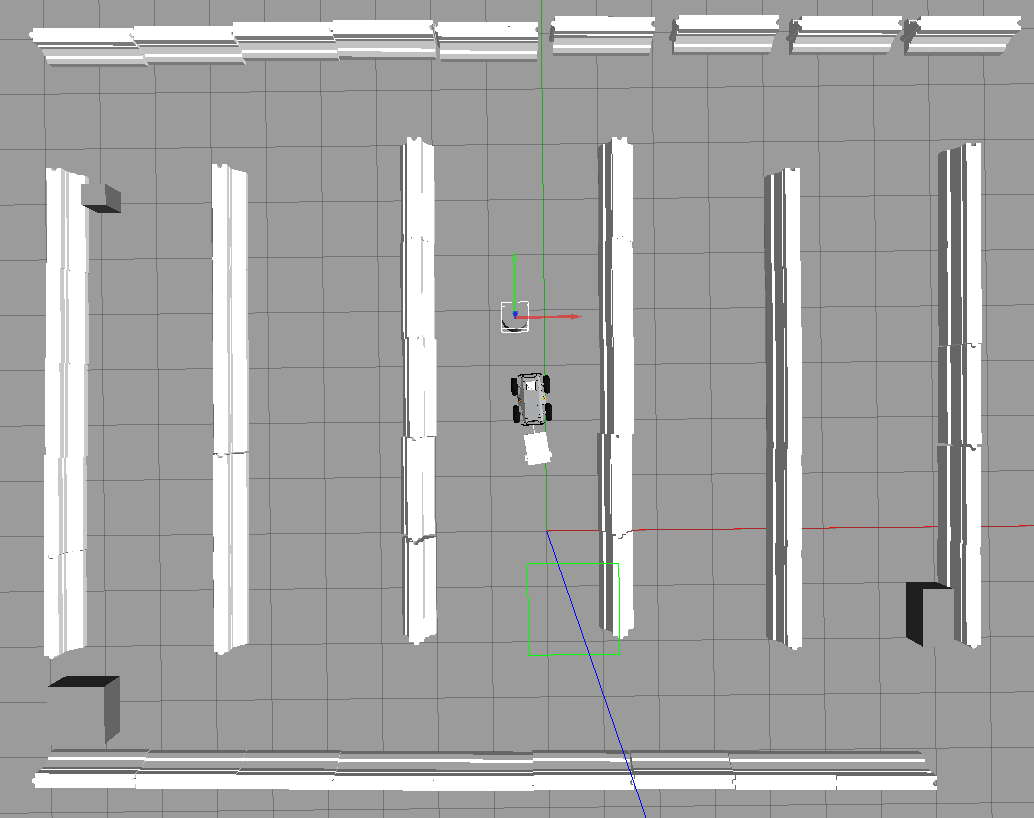
\includegraphics[width=0.85\textwidth]{final_conf.png}
    \caption{Final configuration in the simulated environment. The cilinder was moved and the robot stopped in the parameterised range.}
    \label{fig:sim_obstacle_detection3}
\end{figure}

As observed in figure \ref{fig:sim_obstacle_detection3}, the robot was able to 
detect the obstacle and come to a stop before colliding with it.
\subsection{Real World Results}
\paragraph{} The real world tests results can be shown in an annexed video, however, 
the results were very similar and the robot was able to come to a stop and resume its 
path after the obstacle was removed.

\section{Discussion}
\label{sec:discussion}

\paragraph{}In this section, there will be an overview of the obtained results aswell 
as some insights into the performance of the proposed methods aswell as their viability.

\subsection{Path Tracking}
\paragraph{} When it came to path tracking, if the goal pose was reachable by only moving 
in the forwards direction, the robot would have absolutely no problem reaching it, even with 
the presence of obstacles. However, when the goal pose required a change in direction 
or a hitching manoeuvre, depending on the current configuration of the robot and the 
environment, it couldn't be assured that the robot would be able to reach it. This, 
of course, is due to the fact that the trailer's controller, despite being designed to 
account for such scenarios, struggled when multiple manoeuvres were required in quick 
succession, leading the robot to positions which weren't initialy in the path and could only 
be recovered with a new planning iteration. This fact doesn't invalidate the proposed 
solution as it still provides a successful navigation experience in the majority of 
scenarios and only fails in specific situations where the  robot is in very narrow spaces 
and is required to reverse or in position where the density of voronoi nodes is too low 
to provide a path which avoids the obstacles.

Addressing now the collected data on the tests, a relation of the processing time and the 
length of the path and the length of the recovery segment could be observed. It was found 
that as the length of the path increased, the processing time also increased, which is 
expected as more computations are required to plan and execute longer paths. Also, the processing 
time required for recovery segments was higher than for the dubins segments, meaning that 
paths with similar lengths but one with half the length being Dubins and the other being 
the hybrid A* would have a higher processing time than the one with just the Dubins segments. 
This is also to be expected as the hybrid A* launches additional nodes during the search which 
increases the overall computational load, compared to the Dubins segment which simply calculates 
the mathematical path using a closed-form solution.

% following table has the mean processing time, the mean hybrid length and dubins length and total length 

\begin{table}[H]
    \centering
    \begin{tabular}{|c|c|c|}
        \hline
        \textbf{Test}  & \textbf{Mean Processing Time (ms)} & \textbf{Mean Total Length (m)}\\
        \hline
        Direct Path & 15.914 & 5.232  \\
        \hline
        Obstructed Path & 18.768 & 11.376  \\
        \hline
        Recovery Test & 24.213  & 10.6228  \\
        \hline
    \end{tabular}
    \caption{Mean processing time and lengths of the paths in the simulation tests conducted.}
    \label{tab:mean_processing_time_lengths}
\end{table}
\begin{table}[H]
    \centering
    \begin{tabular}{|c|c|c|}
        \hline
        \textbf{Test}  & \textbf{Mean Processing Time (ms)} & \textbf{Mean Total Length (m)}\\
        \hline
        Direct Path & 59.146 & 8.87  \\
        \hline
        Obstructed Path & 60.678 & 11.885  \\
        \hline
        Recovery Test & 170.196  & 8.858  \\
        \hline
    \end{tabular}
    \caption{Mean processing time and lengths of the paths in the real world tests conducted.}
    \label{tab:mean_processing_time_lengths}
\end{table}

From the collected data, it is possible to assert that the previously mentioned trends hold true, both in 
the simulations as in the real world tests. It was also observed that the recovery process was significantly 
more computationaly complex than the Dubins segments, specialy in the real world tests, where the processing power 
is significantly lower than in the simulation environment. Despite this, the time required to calculate a path proved 
to be fast enough for the allocated task, as it would not be a critical issue in overall performance. Despite this, 
the processing time would still be a factor to consider in future optimizations.

\subsection{Obstacle Detection and Safety}
\paragraph{} The obstacle detection module worked perfectly fine, both in simulation and in the real world, 
with the only aspect to be improved being the time to detect and add the obstacles to the local costmap. However, 
this improvement is outside the scope of this work as it is a standard tool provided by the \gls{NAV2} stack.